
%(BEGIN_QUESTION)
% Copyright 2011, Tony R. Kuphaldt, released under the Creative Commons Attribution License (v 1.0)
% This means you may do almost anything with this work of mine, so long as you give me proper credit

{\bf Flare knockout drum and water seal}

$$\includegraphics[width=15.5cm]{i0002rx01.eps}$$

\underbar{file i0002r}
%(END_QUESTION)





%(BEGIN_ANSWER)


%(END_ANSWER)





%(BEGIN_NOTES)

\filbreak \vskip 20pt \vbox{\hrule \hbox{\strut \vrule{} {\bf Virtual Troubleshooting} \vrule} \hrule}

\noindent
{\bf Predicting the effect of a given fault:} present each of the following faults to the students, one at a time, having them comment on all the effects each fault would produce.

\begin{itemize}
\item{} 
\item{} 
\item{} 
\end{itemize}


\vskip 10pt


\noindent
{\bf Identifying possible/impossible faults:} present symptoms to the students and then have them determine whether or not a series of suggested faults could account for all the symptoms, explaining {\it why} or {\it why not} for each proposed fault:

\begin{itemize}
\item{} Symptom: {\it }
\item{}  -- {\bf Yes/No}
\item{}  -- {\bf Yes/No}
\item{}  -- {\bf Yes/No}
\end{itemize}


\vskip 10pt


\noindent
{\bf Determining the utility of given diagnostic tests:} present symptoms to the students and then propose the following diagnostic tests one by one.  Students rate the value of each test, determining whether or not it would give useful information (i.e. tell us something we don't already know).  Students determine what different results for each test would indicate about the fault, if anything:

\begin{itemize}
\item{} Symptom: {\it LSH-22 registers a high water level in the water seal drum}
\item{} Inspect stem position of LV-21 -- {\bf Yes}
\item{} Check status of LSL-23 -- {\bf No}
\item{} Measure output pressure signal from LT-21 -- {\bf Yes} 
\item{} Check mode (auto/manual) of LC-21 -- {\bf Yes}
\item{} Check output signal value for LC-21 -- {\bf Yes}
\item{} Check reading on PG-37 -- {\bf No}
\item{} Check shutoff valve for instrument air supply -- {\bf No}
\item{} Check to see if the steam trap is clogged -- {\bf No}
\item{} Check reading on PG-36 -- {\bf Yes} (if this gauge is sensitive enough to detect hydrostatic pressure)
\item{} Check status of drain valve to OWS -- {\bf No}
\end{itemize}


\vskip 10pt


\noindent
{\bf Diagnosing a fault based on given symptoms:} imagine the instrument air supply to LC-21 fails (i.e. no air pressure) in this system (don't reveal the fault to students!).  Present the operator's observation(s) to the students, have them consider possible faults and diagnostic strategies, and then tell them the results of tests they propose based on the following symptoms, until they have properly identified the nature and location of the fault:

\begin{itemize}
\item{} Operator observation: {\it LAL-23 activates in the control room}
\item{} Process isolation valves to LT-21 remote seals are both open
\item{} LI-21 registers 0\% level (3 PSI on receiver gauge)
\item{} LC-21 output gauge reads 0 PSI
\item{} LV-21 stem is in the fully {\it shut} position
\end{itemize}



\vskip 10pt

\filbreak



\noindent
{\bf Diagnosing a fault based on given symptoms:} imagine unusually cold weather causes the drain pipe on the knockout drum ``boot'' to freeze, preventing an liquid from exiting the drum into the oily water sewer (don't reveal the fault to students!).  Present the operator's observation(s) to the students, have them consider possible faults and diagnostic strategies, and then tell them the results of tests they propose based on the following symptoms, until they have properly identified the nature and location of the fault:

\begin{itemize}
\item{} Operator observation: {\it LIR-24 high alarm activates in the control room}
\item{} LAH-19 is not active ({\it yet!})
\item{} LG-25 shows completely full of water
\item{} LG-20 shows about 8 inches of water accumulated inside the knockout drum
\item{} LC-24 output gauge reads 1 PSI
\item{} LV-24 stem is in the {\it wide-open} position
\item{} Block valves before and after LV-24 are both open
\end{itemize}



%INDEX% Process: flare knockout drum and water seal (realistic P&ID shown, shared by i00977, i01379, i01608, i02820, i4694)

%(END_NOTES)

